\documentclass{article}

\usepackage{minted}
\usepackage{xcolor}
\usemintedstyle{vs}
\usepackage[utf8]{inputenc}
\usepackage{supertabular}
\usepackage[T1]{fontenc}
\usepackage{icomma}
\usepackage{array} 
\usepackage{color}
\usepackage{amsmath,mathtools}
\usepackage{amssymb,amsfonts}
\usepackage{esint}
\usepackage{multirow}
\usepackage{float}
\usepackage{graphicx}
\usepackage{tikz}
\usepackage[left=2.5cm,right=2.5cm,top=3cm,bottom=3cm]{geometry}
\usepackage{hyperref}
\usepackage[english]{babel}
\usepackage{caption}
\usepackage[bottom]{footmisc}
\usepackage{gensymb}
\usepackage{tabulary}
\usepackage{fancyhdr}
\usepackage{siunitx}
\usepackage{textcomp}
\usepackage[RPvoltages]{circuitikz}
\newcommand{\HRule}{\rule{\linewidth}{0.5mm}}
\usepackage{parskip}
\setlength{\parindent}{20pt}
\setlength{\parskip}{15pt}
\setlength\extrarowheight{2pt}
\usepackage{tcolorbox}
\usepackage{enumitem}
\usepackage[ampersand]{easylist}
\usepackage{subfigure}
\usepackage{hhline}
\usepackage{datetime}
\usepackage{fancyhdr}
\pagestyle{fancy}
\usepackage{lastpage}
\renewcommand\headrulewidth{1pt}
%\usepackage{biblatex} %Imports biblatex package
%\addbibresource{Bibliography.bib} %Import the bibliography file
\usepackage{csquotes}
\usepackage{calligra}
\usepackage{physics}
\usepackage{listings}
\usepackage{xcolor}
\advance\day by -2
\definecolor{codegreen}{rgb}{0,0.6,0}
\definecolor{codegray}{rgb}{0.5,0.5,0.5}
\definecolor{codepurple}{rgb}{0.58,0,0.82}
\definecolor{backcolour}{rgb}{0.95,0.95,0.92}

\lstdefinestyle{mystyle}{
    backgroundcolor=\color{backcolour},   
    commentstyle=\color{codegreen},
    keywordstyle=\color{magenta},
    numberstyle=\tiny\color{codegray},
    stringstyle=\color{codepurple},
    basicstyle=\ttfamily\footnotesize,
    breakatwhitespace=false,         
    breaklines=true,                 
    captionpos=b,                    
    keepspaces=true,                 
    numbers=left,                    
    numbersep=5pt,                  
    showspaces=false,                
    showstringspaces=false,
    showtabs=false,                  
    tabsize=2
}

\lstset{style=mystyle}

\DeclareMathAlphabet{\mathcalligra}{T1}{calligra}{m}{n} 
\DeclareFontShape{T1}{calligra}{m}{n}{<->s*[2.2]callig15}{}
\newcommand{\scripty}[1]{\ensuremath{\mathcalligra{#1}}}

\fancyhead[L]{\textbf{Assignment 4}}
\fancyhead[C]{}
\fancyhead[R]{Selman Tabet - 724009589}
\renewcommand\footrulewidth{1pt}
\fancyfoot[C]{\textbf{Page \thepage/\pageref{LastPage}}}
\fancyfoot[R]{\today}


\begin{document}
\begin{titlepage}
\begin{center}

\includegraphics[scale=1.5]{Figures/TAMUQ.png}
\line(1,0){400}\\
[2mm]
\begin{huge}
\textbf{Assignment 4 Report}\\ 
\end{huge}
\begin{LARGE}
\line(1,0){40}\\
[1.5cm]
ECEN-449-500\\
Microprocessor System Design\\
[3cm]
Assignment 4\\
Lab Report: Timers, Tickers and PWM.\\ 
[2.5cm]
Name: Selman Tabet\\
UIN: 724009589\\
[4cm]
\end{LARGE}
\begin{large}
Electrical and Computer Engineering\\
Texas A&M University at Qatar\\
Spring 2021
\end{large}
\end{center} 
\end{titlepage}

\section*{Overview}
\justify
\large
This assignment required the usage of an EA LPC4088 QuickStart Board mounted on a base board through an FFC cable (basically a ribbon cable, but smaller). Before the board was connected to the computer through a USB 2.0 Micro cable. The online Mbed IDE was used to compile the C code and the output binary files were then copied into the device's flash storage through USB, and leveraging the built-in HDK USB drag-n-drop programming feature to automatically flash the binary file into the board's memory.

This assignment focuses on the usage of the board's timers (including the SysTick interface), tickers and the Pulse-width Modulation (PWM) interface. They are used to schedule tasks in a well-defined manner with respect to time. Timers can be used to count the time elapsed since a certain event with high precision. Tickers are used to define repeated triggers. Finally, PWM is a modulation that can take two parameters, namely the duty cycle and period, to carry out tasks that make use of the modulation scheme, such as motors and LEDs.

Since I have been explicitly prompted to stick to singular short paragraphs to explain my work, many inherent and potentially important nuances will be left out of the discussion and only brief abstractions of the programs' workings would be explained.\pagebreak

\section*{Question 1}
\begin{minted}{cpp}
/* Selman Tabet (@selmantabet - https://selman.io/) - UIN 724009859
Assignment 4 - Question 1

This function leverages the board's SysTick timer to turn LEDs between two
states, one where LEDs 2, 3 and 4 turn on for two seconds, the other state 
turns LED1 and would switch on and off every half a second, for a period of two
seconds. Which means that LED1 would be blinking twice through that period.
The board's clock rate is 120MHz, and since the reload register is 24 bits wide
the maximum value that can be used is around 16.7 million. Thus, the value of
15 million cycles was used for the SysTick implementation here. Being set at 
8th of a second, this reload value would result in eight ticks per second.

Developed using the Mbed IDE. Tested on an EA LPC4088 QuickStart Board. */

#include "mbed.h"

#define STCTRL             (*((volatile unsigned long *) 0xE000E010))
#define STRELOAD           (*((volatile unsigned long *) 0xE000E014))
#define STCURR             (*((volatile unsigned long *) 0xE000E018))

DigitalOut my_led1(LED1); //Active Low
DigitalOut my_led2(LED2); //Active Low
DigitalOut my_led3(LED3); //Active High
DigitalOut my_led4(LED4); //Active High

int ticks = 0; //To keep track of SysTicks done so far.
int state_id = 0; //Zero = LEDs 2-3-4 ON, One = LED1 ON and blinking. 

extern "C" void SysTick_Handler(void){ //SysTick interrupt handler
    ticks++; //tick!
    if (ticks > 15){ //Two seconds (AKA 16 ticks) elapsed, switch states.
        ticks = 0; //Ticks reset.
        if (state_id == 0){ //Switch to LED1 ON.
            my_led2 = 1; my_led3 = 0; my_led4 = 0;
            my_led1 = 0;
        }
        else { //Switch to LED2,3,4 ON.
            my_led2 = 0; my_led3 = 1; my_led4 = 1;
            my_led1 = 1;
        }
        state_id = !state_id; //State alternated.
    }
    else { //Turn ON/OFF every 4 ticks, i.e. every half a second.
        if ((state_id == 1) && (ticks%4 == 0)) my_led1 = !my_led1;
    }
}

int main(void){
    my_led1 = 1; my_led2 = 0; my_led3 = 1; my_led4 = 1; //Default state.
    SystemInit(); //Initialize the oscillator (PLL) on the MCU.
    
    STCTRL |= 0x1 << 0; //Enable system tick counter (bit 0)
    STCTRL |= 0x1 << 1; //Enable system interrupt (bit 1)
    STCTRL |= 0x1 << 2; //Select CPU clock as source (bit 2)
    
    /*Core_clk is 120MHz (which was unspecified in the handout btw -.-)
    Since the max value to reload is almost 17m due to bit-width limitation,
    15m is a choice that would make subsequent tick-related calculations 
    far more convenient.
    
    Half a second = 4 ticks. One second = 8 ticks. Two seconds = 16 ticks.*/
    int RELOAD_VAL = SystemCoreClock/8; //15 million cycles == 8th of a second

    STRELOAD = RELOAD_VAL;
    while(1); //Run forever.
}
\end{minted}


This function leverages the board's SysTick timer to turn LEDs between two states, one where LEDs 2, 3 and 4 turn on for two seconds, the other state turns LED1 and would switch on and off every half a second, for a period of two seconds. Which means that LED1 would be blinking twice through that period.
The board's clock rate is 120MHz, and since the reload register is 24 bits wide, the maximum value that can be used is around 16.7 million. Thus, the value of 15 million cycles was used for the SysTick implementation here. Being set at 8th of a second, this reload value would result in eight ticks per second.\pagebreak



\section*{Question 2}
\begin{minted}{cpp}
/* Selman Tabet (@selmantabet - https://selman.io/) - UIN 724009859
Assignment 4 - Question 2

This function uses the board's built-in timer to measure the amount of time
a user pressed a button. The timer starts upon a button press, and is stopped
upon a button release. The measured time is then printed into through the
board's Serial port.

Developed using the Mbed IDE. Tested on an EA LPC4088 QuickStart Board. */

#include "mbed.h"

Serial pc(USBTX, USBRX); //Serial channel over HDK USB interface
Timer swatch; //Define timer object
InterruptIn button(p23); //Define the pushbutton as an interrupt

void isr1(void){
    swatch.start(); swatch.reset(); //Start and reset timer to zero
    }
    
void isr2(void){ //Stop and measure time elapsed then print via the Serial port
    swatch.stop();
    pc.printf("Pushbutton pressed for %f seconds!\n", swatch.read());
    }

int main(){
    button.mode(PullUp); //Enable pullup resistor
    button.fall(&isr1); //Register an ISR on the falling edge
    button.rise(&isr2); //Register an ISR on the rising edge
    pc.printf("Selman Tabet’s Stopwatch:\n");
    while(1); //Run forever.
}
\end{minted}
\pagebreak


This function makes use of the board's built-in timer to measure the amount of time a user pressed a button. Two ISRs were defined; one that would be triggered when the button is pressed so it starts counting, and the other is triggered when the button is released so that the timer is stopped and measured. The measured time is then printed through the board's Serial port. Figure \ref{fig:q2} includes a screenshot of the terminal's output on multiple button presses.


\begin{figure}[!ht]
\begin{center}
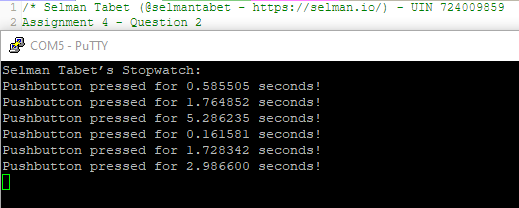
\includegraphics{Figures/Q2.png}
\end{center}
\caption {PuTTY Terminal displaying the board's timer output through its Serial COM port.}
\label{fig:q2}
\end{figure}

\pagebreak


\section*{Question 3}
\begin{minted}{cpp}
/* Selman Tabet (@selmantabet - https://selman.io/) - UIN 724009859
Assignment 4 - Question 3

This function uses the board's ticker interface to switch LEDs every second.
Only one LED would be on at any given time. The sequence is defined as:
LED1 - LED2 - LED3 - LED4
This sequence is done three times in a cyclic manner, then the sequence is 
reversed for another three times, and then back to normal for another three,
and so on.

Developed using the Mbed IDE. Tested on an EA LPC4088 QuickStart Board. */

#include "mbed.h"

Ticker led_flipper; //Define ticker object

DigitalOut my_led1(LED1); //Active Low
DigitalOut my_led2(LED2); //Active Low
DigitalOut my_led3(LED3); //Active High
DigitalOut my_led4(LED4); //Active High

int state_id = 1; //LED Sequence 1-2-4-3 (State 1, 2, 3 and 4, respectively).
int iterator = 0; //To determine the number of turns done so far
int invert_flag = 0; //Clockwise (CW) Vs. Anticlockwise (ACW) ** CW = 0 **

void ledToggle () {
    switch(state_id){
        case 1:
            my_led1 = 0; //LED1 ON
            my_led2 = 1; my_led3 = 0; my_led4 = 0; //Rest of the LEDs OFF.
            if (invert_flag == 1){ //Edge case, a dead-end on ACW turn.
            /*Check if the third turn was completed to invert the direction
            and reset the iterator, otherwise, count as a new turn (iterator
            incremented) and force state 4.*/
                if (iterator == 2) {iterator = 0; invert_flag = 0;}
                else {iterator++; state_id = 4;} //Lap complete, force state 4.
            }
            else state_id++; //Move to state 2.
            break;
        case 2:
            my_led2 = 0; //LED2 ON
            my_led1 = 1; my_led3 = 0; my_led4 = 0; //Rest of the LEDs OFF.
            //Check direction then move accordingly.
            if (invert_flag == 0) state_id++; 
            else state_id--;
            break;
        case 3:
            my_led4 = 1; //LED4 ON
            my_led1 = 1; my_led2 = 1; my_led3 = 0; //Rest of the LEDs OFF.
            //Check direction then move accordingly.
            if (invert_flag == 0) state_id++;
            else state_id--;
            break;
        case 4:
            my_led3 = 1; //LED3 ON
            my_led1 = 1; my_led2 = 1; my_led4 = 0; //Rest of the LEDs OFF.
            if (invert_flag == 0){ //Edge case, a dead-end on CW turn.
            /*Check if the third turn was completed to invert the direction
            and reset the iterator, otherwise, count as a new turn (iterator
            incremented) and force state 1.*/
                if (iterator == 2) {iterator = 0; invert_flag = 1;}
                else {iterator++; state_id = 1;}
            }
            else state_id--;
            break;
        default:
            state_id = 1; //meh, irrelevant to this FSM. 
            //Effective for error handling though :)
    }
}

int main(){
    my_led1 = 1; my_led2 = 1; my_led3 = 0; my_led4 = 0; //All OFF.
    
    led_flipper.attach(&ledToggle, 1.0); //Call ledToggle every second.
    
    while(1); //Run forever.
}
\end{minted}
\pagebreak

This function uses the board's ticker interface to switch LEDs every second. Only one LED would be on at any given time. The LEDs are turned on then off in the following sequence: \texttt{LED1 -> LED2 -> LED3 -> LED4}.
This sequence is done three times in a cyclic manner, then the sequence is reversed for another three times, and then back to normal for another three, and so on. To achieve this behavior, three variables were defined; 

\begin{itemize}
  \item \texttt{iterator} : Counts how many turns out of three were taken so far.
  \item \texttt{state\_id} : Keeps track of which LED is ON, i.e. the current state.
  \item \texttt{invert\_flag} : Defines the direction at which the sequence is being executed.
\end{itemize}

\pagebreak

\section*{Question 4}
\begin{minted}{cpp}
/* Selman Tabet (@selmantabet - https://selman.io/) - UIN 724009859
Assignment 4 - Question 4

This function uses the PWM interface to control the duty cycle and period of
LED1. The duty cycle defines how much, in percentage, of a period does a 
does the board send a logical HIGH signal to the LED. Given that LED1 is
Active Low, that would translate into how much of a time period would the LED
be off.

A short button press would result in a slight increase to the duty cycle,
while a press that is longer than 3 seconds would result in an increase in
the period. When the maximum duty cycle value is reached (1.0f or 100%), the
next short press would result in its reset to 0.0f. This same approach is taken
for the time period, as the limit of 5 seconds is reached, it would be reset to
one second on a long press.

Developed using the Mbed IDE. Tested on an EA LPC4088 QuickStart Board. */

#include "mbed.h"

Serial pc(USBTX, USBRX); //Serial channel over HDK USB interface
Timer swatch; //Define timer object
InterruptIn button(p23);

PwmOut my_led1(LED1); //Define LED1 as PWM output (Active Low)
DigitalOut my_led2(LED2); //Active Low
DigitalOut my_led3(LED3); //Active High
DigitalOut my_led4(LED4); //Active High

float period = 2.0f; //Initial period
float duty_cycle = 0.50f; //Initial duty cycle


void isr1(void){ //Start counting
    swatch.start(); swatch.reset(); //Start and reset timer to zero
    }

void isr2(void){
    swatch.stop(); //Stop counting and measure to see which action to take
    if (swatch.read() < 3.0f){
        if (duty_cycle >= 1.0f) duty_cycle = 0.0f; //Duty cycle reset
        else duty_cycle += 0.1f; //Increment duty cycle by 10%
        my_led1.period(period); //Enforce new PWM parameters
        my_led1.write(duty_cycle);
        pc.printf("LED1 PWM Duty Cycle: %f\n", duty_cycle);
    }
    else {
        if (period >= 5.0f) period = 1.0f; // >= because of an IEEE 754 quirk
        else period += 1.0f; //Increment period by 100ms
        pc.printf("LED1 Period: %f seconds\n", period);
        my_led1.period(period); //Enforce new PWM parameters
        my_led1.write(duty_cycle);
    }
}

int main(){
    button.mode(PullUp); //Initialize button resistor.
    pc.printf("Selman Tabet’s PWM Controller:\n");
    my_led2 = 1; my_led3 = 0; my_led4 = 0; //All LEDs (except LED1) OFF
    my_led1.period(period); //Period set to two seconds at the start
    my_led1.write(duty_cycle); //Initially set to 50%
    
    button.fall(&isr1); //Register an ISR on the falling edge
    button.rise(&isr2); //Register an ISR on the rising edge
    
    while(1); //Run forever.
}
\end{minted}
\pagebreak

This function uses the PWM interface to control the duty cycle and period of \texttt{LED1}. The duty cycle defines how much, in percentage, of a period does a does the board send a logical HIGH signal to the LED. Given that \texttt{LED1} is Active Low, that would translate into how much of a time period would the LED be OFF. A short button press would result in a slight increase in the duty cycle, while a press that is longer than 3 seconds would result in an increase in the period. When the maximum duty cycle value is reached (\texttt{1.0f} or 100\%), the next short press would result in its reset to \texttt{0.0f}. This same approach is taken for the time period; as the limit of 5 seconds is reached, it would be reset to one second on a long press. Figure \ref{fig:q4} is a screenshot reflecting the PWM parameter changes upon different button presses.

\begin{figure}[!ht]
\begin{center}
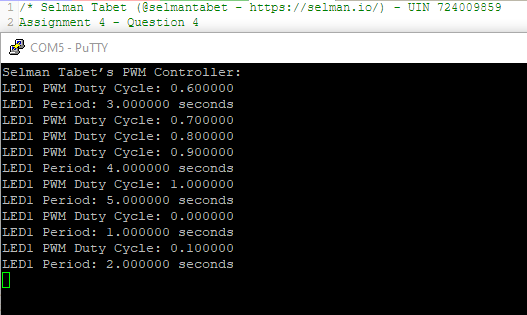
\includegraphics{Figures/Q4.png}
\end{center}
\caption {PuTTY Terminal displaying changed PWM parameters upon button presses.}
\label{fig:q4}
\end{figure}

\end{document}

